% Chapter 5

\chapter{\uppercase{Dataset, Fine-Tuning, Results and Status}}
\label{ch:results}
This chapter covers the data, the fine-tuning, a demo, our results so far and what is
left to do.

\section{\uppercase{Datasets}}
Each training row has the same shape: the input is a short conversation plus a task
(extract, consolidate or reflect), and the output is the expected memory, i.e. assertions,
inferences or an answer, each tied to a source quote. For example in the Maya
episode the user says ``I live in Chennai.'' and later ``Bengaluru is now my home city.'',
and the expected output is the assertion ``Maya, home city, Bengaluru'' with
\code{correction:true}, \code{source:user} and that quote. The training rows and prompts keep
the wording the model was trained on (kinds \code{fact} and \code{observation}, the heading
``Existing facts:''); the service translates these to \code{attribute} and \code{inference} at the
model boundary, so the renaming used in this report does not change the model's contract.

The fine-tuning data started out as only coding conversations and we later expanded
it to 16 domains (family, food, travel, education, work, software and so on). All
conversations are synthetic. They were generated by the teacher model GPT-5.6-sol,
cross-checked by a second adversarial model and then cleaned. In total there are 2,961
task examples, split into 2,095 for training, 424 for validation and 442 for testing.
Figure~\ref{fig:domains} shows the spread across domains. Software and technical projects is the
biggest with 240 rows and the rest have roughly 110 to 140 each. (Several tasks can come
from one episode, so this counts rows, not conversations.)

\begin{figure}[H]
\centering
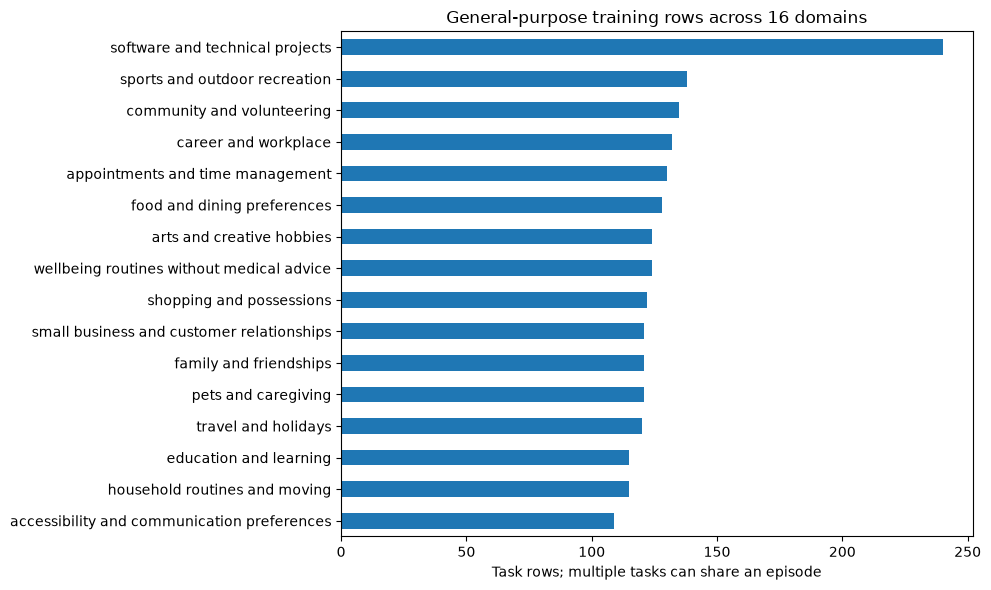
\includegraphics[width=0.85\textwidth,height=0.26\textheight,keepaspectratio]{figures/fig5_1_domains.png}
\caption{General-purpose training rows across the 16 domains}
\label{fig:domains}
\end{figure}

A lot of the rows test whether the model keeps only what the user actually said. For
example, the assistant says ``You could learn violin this winter.'' and the user replies
``No, that is not my plan. I am learning watercolor painting.'' The expected memory is
just that the user is learning watercolor painting. The assistant's suggestion should not
become a memory.

For testing outside our own data distribution we used LoCoMo \cite{maharana2024locomo}, which has
real-style conversations over many sessions. We took 16 conversation segments from 10
conversations, with 40 reference assertions. A typical one is Caroline and Melanie chatting
about a pottery class and a painting; the expected memory is that Melanie made a plate
in pottery class and Caroline painted a picture inspired by her beach visit.

\section{\uppercase{Fine-Tuning and Model Selection}}
The model is Qwen3-4B-Instruct-2507, fine-tuned with QLoRA \cite{dettmers2023qlora} and served
through Ollama. Following Figure~\ref{fig:m5}, GPT-5.6-sol labelled the episodes for the extract,
consolidate and reflect tasks, every label was checked for structure and source quotes (and
repaired if needed), and the valid ones were frozen into the 2,095/424/442 split. Rows
were tokenised with a 4,096 token limit and the prompt was masked so only the target
is supervised. Training used QLoRA on the frozen base with NF4 quantisation and rank
16, going from Stage A to Stage B. The adapter was then merged and quantised to a
Q8\_0 GGUF with llama.cpp, compared against the base model on 64 internal tasks and
16 external cases, checked live (retain, graph, recall/reflect), and packaged with a
SHA-256 checksum and imported into Ollama as \code{mem-extractor:general-v1}.

We actually started with Qwen3-1.7B. It was fine on synthetic examples but bad on
natural conversations, only 18 of 33 extraction windows passed validation even after
refinement. Most failures were wrong source attribution, quotes that didn't match and
invalid IDs. That's what pushed us to broaden the training data, tighten the output
constraints and move up to the 4B model.

\section{\uppercase{Live Demonstration}}
The demo follows the same idea as Maya (record, ask later in a new session, see the
correction) but with its own values: a certificate expiry date, a weekly review time, a
dashboard owner, and later a release-freeze time. Figure~\ref{fig:demo-a} shows the first two
steps.

\begin{figure}[H]
\centering
\begin{minipage}[t]{0.49\textwidth}
\centering
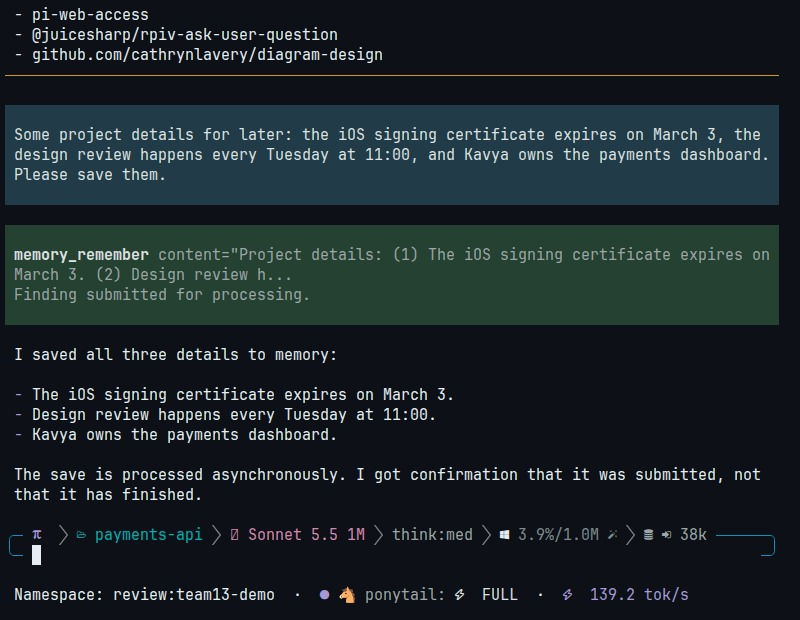
\includegraphics[width=\textwidth]{figures/fig5_2_recording.jpg}\\
\small (a) Recording in the first session
\end{minipage}\hfill
\begin{minipage}[t]{0.49\textwidth}
\centering
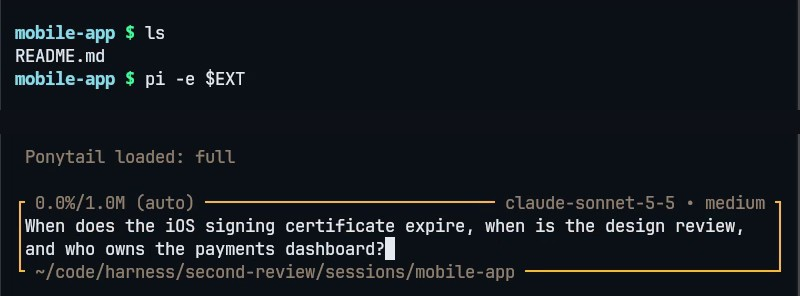
\includegraphics[width=\textwidth]{figures/fig5_3_new_session.jpg}\\
\small (b) Asking in a new session
\end{minipage}
\caption[Demo: recording details, then recalling them in a new session]{(a) The user gives a certificate expiry date, a weekly review time and the
dashboard owner, which are submitted for memory processing. (b) A fresh session in
another project directory asks for the same details without repeating them}
\label{fig:demo-a}
\end{figure}

In (a) the agent calls the \code{memory\_remember} tool and notes that processing is
asynchronous, so it can't confirm storage yet. In (b) a new session in \code{mobile-app} (not
\code{payments-api}) asks for all three without restating them, like Maya asking E5.

\begin{figure}[H]
\centering
\begin{minipage}[t]{0.49\textwidth}
\centering
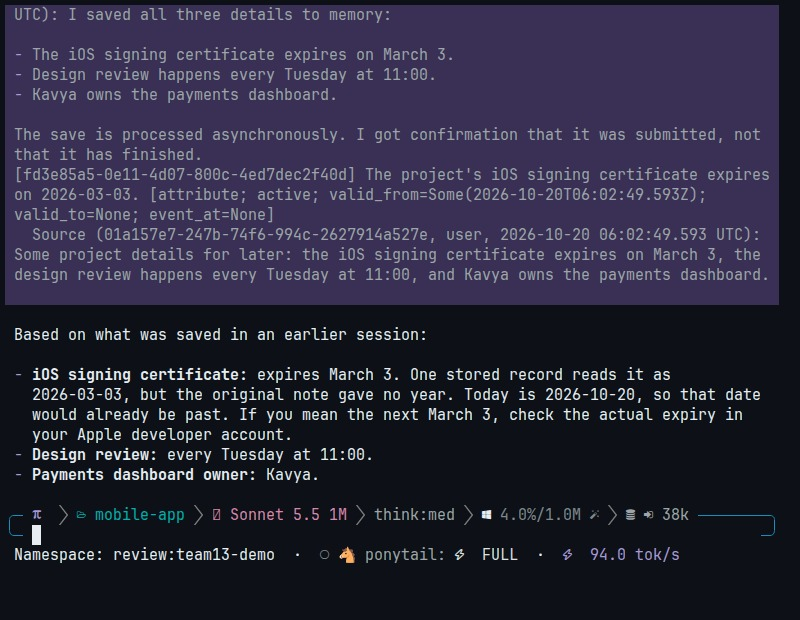
\includegraphics[width=\textwidth]{figures/fig5_4_recall.jpg}\\
\small (a) Recalled answer
\end{minipage}\hfill
\begin{minipage}[t]{0.49\textwidth}
\centering
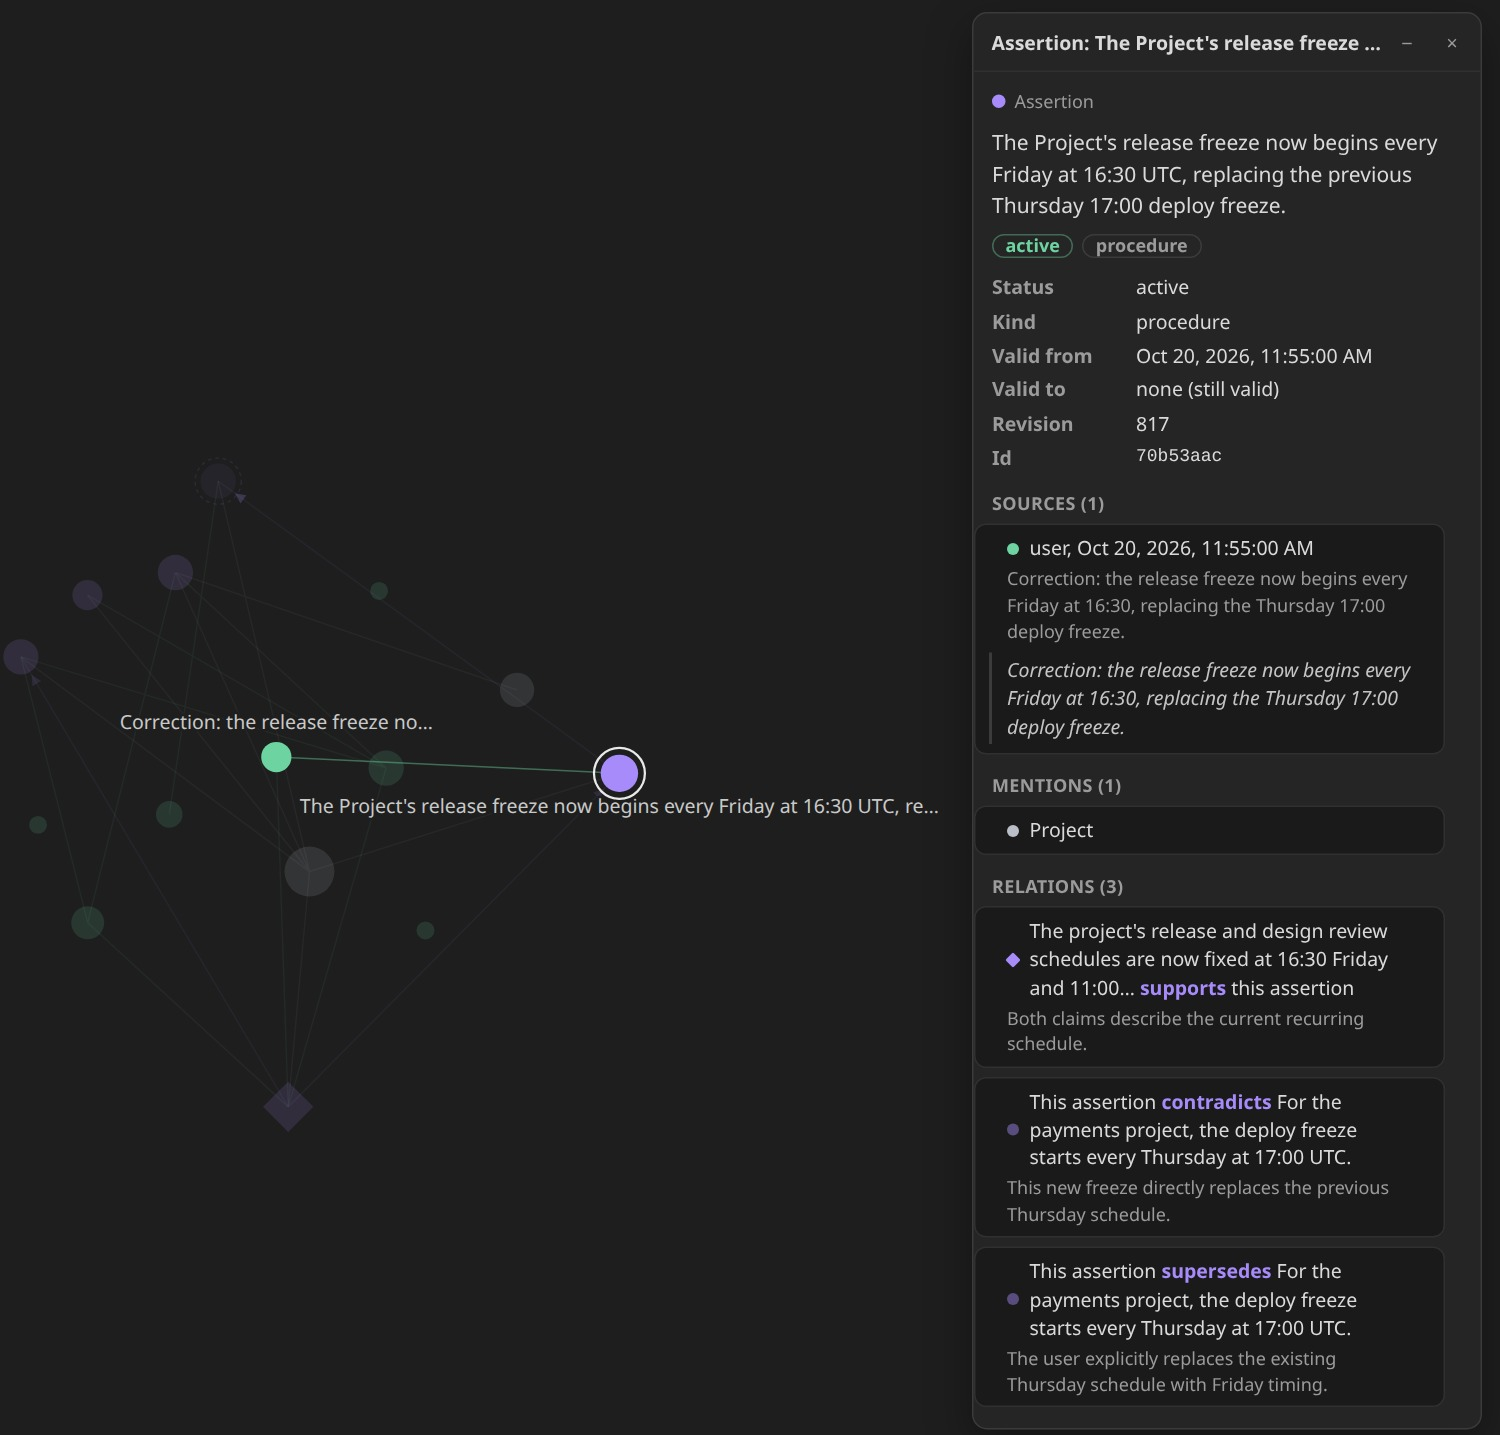
\includegraphics[width=\textwidth]{figures/fig5_5_graph.jpg}\\
\small (b) Corrected assertion in the graph
\end{minipage}
\caption[Demo: recalled answer and the corrected assertion in the graph]{(a) Memory from the first session is added to the context and the agent
answers March 3, Tuesday at 11:00 and Kavya. (b) The graph shows Friday at 16:30 as
the current release-freeze time, linked to the previous Thursday at 17:00 value, with the
supporting message and history in the side panel}
\label{fig:demo-b}
\end{figure}

In Figure~\ref{fig:demo-b}(a) the agent answers from the recalled assertions (March 3, since no year was
given, then Tuesday 11:00 and Kavya) and says the information came from an earlier
session. It also notes that the extracted assertion stored the date as 2026-03-03 although
the user gave no year, which shows why answers cite their source quotes. In (b) the Friday 16:30 freeze is
linked to the old Thursday 17:00 value by \code{contradicts} and \code{supersedes}, same as
Bengaluru and Chennai.

\section{\uppercase{Results and Findings}}
Most of what we know so far comes from the demos, a database audit and the model
comparison.

In a three-session coding demo the required output changed from milliseconds to
microseconds partway through. In the next session the system passed this on to the agent
without the user repeating it, and the agent used microseconds. In another test
conversation we gave a person's city and food preference and then changed only the city.
The system used the new city, kept the old one as history, and still had the food
preference.

The database audit found that all 142 stored source quotes matched their original text
exactly, though a matching quote doesn't prove the model understood it correctly. It
also found 8 inferences, each linked to at least two supporting assertions. Dates are still
weak: a message sent on June 1 said ``tomorrow'' and the system read it as June 3.

Table~\ref{tab:comparison} compares Qwen3-4B before and after fine-tuning, on 64 unseen tasks
across the 16 domains and on 16 external conversation samples.

\begin{table}[H]
\caption{Qwen3-4B before and after fine-tuning}
\label{tab:comparison}
\centering
\begin{reporttable}
\begin{tabularx}{\textwidth}{|Y|c|c|}
\hline
\multicolumn{1}{|c|}{\textbf{Measurement}} & \textbf{Before} & \textbf{After} \\
\hline
Correctly combined related assertions & 1/16 & 13/16 \\
\hline
Correct answers from supplied memories & 10/16 & 15/16 \\
\hline
Expected assertions recovered & 50/55 & 41/55 \\
\hline
Extracted claims supported by the source & 92.1\% & 90.5\% \\
\hline
Corrections handled correctly & 8/8 & 8/8 \\
\hline
Outputs passing format checks & 64/64 & 63/64 \\
\hline
Expected assertions recovered (16 external samples) & 16/40 & 13/40 \\
\hline
\end{tabularx}
\end{reporttable}
\end{table}

Combining assertions and answering clearly got better (1/16 to 13/16 and 10/16 to 15/16),
and corrections were right in all 8 cases both times. But extraction got worse. Assertions
recovered dropped from 50/55 to 41/55 internally and 16/40 to 13/40 on the external
samples, supported claims dipped a bit from 92.1\% to 90.5\%, and one output failed the
format check. Honestly this was a bit disappointing and we haven't fully figured out
why yet. Passing the format check also says nothing about whether the extracted assertions are right
(the June 1 date passed it). Since the full benchmark isn't done, we can't claim an overall improvement on
long conversation histories yet.

\section{\uppercase{Status and Pending Work}}
M1 is implemented and covered by the Pi integration tests (capture, retries, namespace
changes). M2 is implemented but its extraction quality still needs work. M3 is
implemented, with integration tests for validity intervals, conflicts, invalidation and
graph cleanup, but needs testing on harder updates. M4 is implemented and has
retrieval tests and live checks, but the full benchmark is pending. For M5, training and
integration are done and evaluation is still going on. The pending items for each
module are listed in the next section.

\section{\uppercase{Conclusion and Future Work}}
We built all five modules of the memory engine: source capture, assertion extraction and
consolidation, temporal graph management, hybrid retrieval with grounded answers,
and model training. Four are implemented and M5 is trained and integrated with
evaluation still going on. In the demos and audit, information from one session was
recalled in a new one, a corrected assertion was stored with its history without touching
unrelated assertions, and all 142 source quotes matched. Fine-tuning helped a lot with
combining assertions (1/16 to 13/16) and answering from retrieved memories (10/16 to
15/16).

Some things aren't there yet. Extraction regressed after fine-tuning (50/55 to 41/55
internal, 16/40 to 13/40 external), relative dates are sometimes wrong, and without the
full LongMemEval-S run we can't say it's better over long histories. Future work, by
module:
\begin{itemize}[itemsep=0pt]
\item M1: API access control and verified backup and restore.
\item M2: better coverage of missed assertions, date interpretation and source attribution;
measure the review step's quality and latency.
\item M3: evaluate ambiguous updates, aliases and longer correction histories.
\item M4: finish LongMemEval-S, compare graph and consolidation ablations, report
retrieval quality and latency.
\item M5: fix the extraction regression and date errors, more external testing and
independent human review.
\end{itemize}
